\documentclass{article}
\usepackage[margin=1.5cm]{geometry}
\usepackage{microtype} % Slightly better kerning
\usepackage{graphicx}
\graphicspath{ {./figs/} }
\usepackage[colorlinks=true]{hyperref}
\setlength\parindent{0pt}

\usepackage{array }% New env. for equation conditions where aligned
\newenvironment{conditions}[1][where:] 
  {#1 \begin{tabular}[t]{>{$}l<{$} @{${}={}$} l}}
  {\end{tabular}\\[\belowdisplayskip]}

\usepackage{tikz}
\usepackage{pgfplots}

\title{Spatial Interpolation Notes}

\begin{document}
\maketitle

\section{Introduction}

We want to use interpolation because it is reasonable to assume that spatially distributed variables are also spatially correlated.
It is not always true, but often worth exploring as part of an analysis.
There are multiple different methods to interpolate data that depend on different underlying assumptions.
These methods are described below.

\begin{center}
    \fbox{Information from \href{https://desktop.arcgis.com/en/arcmap/10.3/tools/3d-analyst-toolbox/how-kriging-works.htm}{ARCGIS} unless listed otherwise}
\end{center}

\section{Inverse distance weighting (IDW)}

IWD determines cell values using a linearly weighted combination of surrounding values.
The weights are function of the inverse distance.
The general form for the IDW function is:

\[\hat{Z}(s_{0})= \frac{\sum_{i=1}^{n} w (s_{i}) Z (s_{i})}{\sum_{i=1}^{n} w (s_{i})}\]

\begin{conditions}
    w(s_{i}) & $||s_{i} - s_{0}||^{-p}$ \\
    || \cdot || & Euclidean distance \\
    p & an inverse distance weighting power, defaulting to 2
\end{conditions}

The value of $p$ determines how much closer values are preferred.
As $p$ increases, IDW approaches a one-nearest-neighbour interpolation model.
$p$ can be selected using cross-validation.

Another way to control IWD interpolation is through selecting the number of neighbouring observations to include.
This can improve speed of interpolation, and may be used when there is reason to believe that distant points have little correlation.
There are two approaches for varying the number of points used for interpolation:

\begin{enumerate}
    \item Varying search radius 
    \begin{itemize}
        \item The number of points to include is fixed, and the radius changes to include that set number
        \item Depends on the density of observations fluctuating
        \item The maximum radius can also be set, in which case all points will be included if that max radius is reached before $n$
    \end{itemize}
    \item Fixed search radius
    \begin{itemize}
        \item Set a radius and minimum number of points
        \item If $n <$ minimum number of points at set radius, the radius increases until the minimum is reached.
    \end{itemize}
\end{enumerate}

In addition to these two approaches, barriers can be created to limit the searches for neighbouring points, i.e. only search for this side of a river.

\section{Kriging}

Kriging is a way to interpolate data and estimate a surface for geospatial data.
There are two main ways of doing this:

\begin{itemize}
    \item Inverse distance weighting (IDW) and spline methods
    \item Kriging
\end{itemize}

IDW are deterministic interpolation methods as they are directly based on the surrounding values or smoothed formulas.
Kriging is different as it uses autocorrelation and takes position into account in the statistical models.
Kriging uses a certain number of neighbouring points, or all points within a specified radius (cf kNN).

The general formula for IDW and kriging is:

\[\hat{Z}(s_{0} )=\sum_{i=1}^{N}\lambda_{i} Z (s_{i})\]

\begin{conditions}
Z \left(s_{i}\right) & the measured value at the $i$th location \\
\lambda_{i} & an unknown weight for the measured value at the $i$th location \\
s_{0} & the prediction location \\
N & the number of measured values
\end{conditions}

The difference between IDW and kriging is that in IDW, $\lambda_{i}$ only depends on distance to prediction location.
In kriging $\lambda_{i}$ also depends on autocorrelation i.e. spatial relationship between prediction locations.

\subsection{Assumptions in kriging}

\begin{center}
    \fbox{Information for subsection from \href{https://www.publichealth.columbia.edu/research/population-health-methods/kriging-interpolation}{Columbia}}    
\end{center}

For kriging to be used, there are a number of assumptions/conditions to be met.
These conditions can be checked in exploratory data analysis.

\begin{enumerate}
    \item The data should be stationary
    \begin{itemize}
        \item Means that the joint probability distribution does not vary across the study space, so the same parameters (e.g. mean, range and sill etc) are valid across the space
        \item Means one variogram is valid across the space
    \end{itemize}
    \item Assumption of isotropy
    \begin{itemize}
        \item Uniformity in all directions (semivariance identical in all directions)
    \end{itemize}
\end{enumerate}



\section{Creating a prediction map with kriging}

There are two steps:

\begin{enumerate}
    \item Create the variograms and covariance functions to estimate the spatial autocorrelation values that depend on the model of autocorrelation (fitting a model).
    \item Predict the unknown values
\end{enumerate}

\subsection{Variography (spatial modelling/structural analysis)}

There are often too many pairs of spatial points to calculate and plot the distance for each pair.
Instead, spatial distances are put into lag bins i.e. all points in the range $40m < x \le 50m$ of point A, and calculate the semivariance.
The semivariance is equal to half the variance of the differences between all possible points spaced a constant distance apart.

\[\gamma (h) = \frac{1}{2}[z(x_{i}) - z(x_{j})]^2\]

Plotting the distance vs semivariance produces an empirical semivariogram.
Closer items should be more similar, therefore lower semivariance.
The opposite is true for further points.

A model is fit to the empirical semivariogram (cf regression).
Different types of models can be fit the the semivariogram:

\begin{itemize}
    \item Spherical (most common)
    \item Circular
    \item Exponential
    \item Gaussian
    \item Linear
\end{itemize}

\begin{figure}[h]
    \centering
    \caption{Different types of models used in spatial modelling \href{https://www.publichealth.columbia.edu/research/population-health-methods/kriging-interpolation}{(Poilou 2008)}. a) Linear semi-variogram; (b) spherical semi-variogram; (c) exponential semi-variogram; and (d) power semi-variogram}
    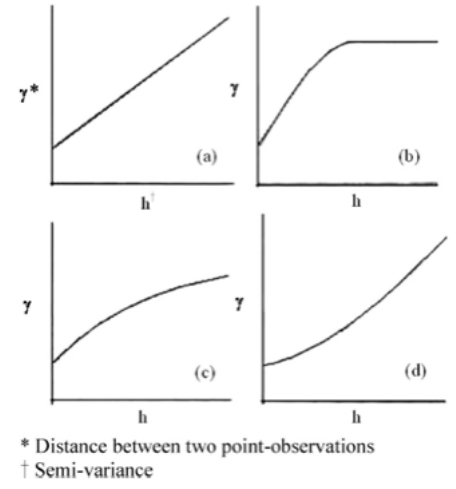
\includegraphics[width=10cm]{semivariogram-models.png}
\end{figure} 

There are a number of key points on the figures:

\begin{itemize}
    \item Range
    \begin{itemize}
        \item The Range is the point at which the semivariance first levels off
        \item Items within the range are autocorrelated (distance matters)
        \item Items outside the range are not autocorrelated (distance no longer changes the semivariance)
    \end{itemize}
    \item Sill 
    \begin{itemize}
        \item The Sill is the height at which the semivariance levels off to
    \end{itemize}
    \item Nugget
    \begin{itemize}
        \item The minimum value of semivariance ($\gamma (h = 0)$)
        \item Theoretically there is no semivariance when $h=0$, but in reality it is present due to measurement error or spatial sources of variation at distances smaller than the sample interval (or both)
    \end{itemize}
    \item Partial Sill
    \begin{itemize}
        \item Amount of semivariance between Sill and the Nugget
    \end{itemize}
\end{itemize}

\subsection{Predictions}

Now a model has been fit to the semivariance and autocorrelation can be observed, predictions can be made within the domain.
Kriging differs from IWD as it uses the semivariogram to calculate the weights.
There are two methods used in kriging:

\begin{enumerate}
    \item Ordinary kriging
    \begin{itemize}
        \item Assumes the constant mean is unknown
    \end{itemize}
    \item Universal kriging
    \begin{itemize}
        \item Assumes there's a prevailing trend
        \item Trend is modelled with polynomial function, and subtracted from observed
        \item Semivariogram is modelled on the residuals to produce autocorrelations
    \end{itemize}
\end{enumerate}

\end{document}